\documentclass[12pt]{article}

\usepackage[margin=2cm]{geometry}

% BibTeX setup
\usepackage[backend=bibtex, bibstyle=alphabetic, citestyle=alphabetic]{biblatex}
\bibliography{references}

\usepackage[english]{babel} % English

% Standard packages for math-related things.
\usepackage{amsmath}
\usepackage{amssymb}
\usepackage{amsthm}
\usepackage{mathtools}

\usepackage{graphicx} % to include graphics with \includegraphics[options]{imagefile}

\theoremstyle{plain} % Usual style for theorems, etc.
\newtheorem{theorem}{Theorem}
\newtheorem{lemma}[theorem]{Lemma}
\newtheorem{corollary}[theorem]{Corollary}

\newcommand{\N}{\mathbb{N}} % blackboard bold N for natural numbers
\newcommand{\R}{\mathbb{R}} % blackboard bold R for real numbers
\newcommand{\Z}{\mathbb{Z}} % blackboard bold Z for integers

\newcommand{\set}[1]{\{#1\}}

\begin{document}

\begin{lemma}
A string graph can be realized by a family of polygonal arcs with a finite number of intersections.
\end{lemma}

\begin{proof}
Assume string graph realized by \( (C_i)_{i\in I} \). Let \(C = \bigcup_{i\in I} C_i\).
\(C\) is compact since it is bounded and closed. Let \(p \in C\) and \(O \ni p\) an open neighborhood 
in the plane. \(O\) \textit{respects} the family of curves if \(O\) only intersects curves that contain \(p\).

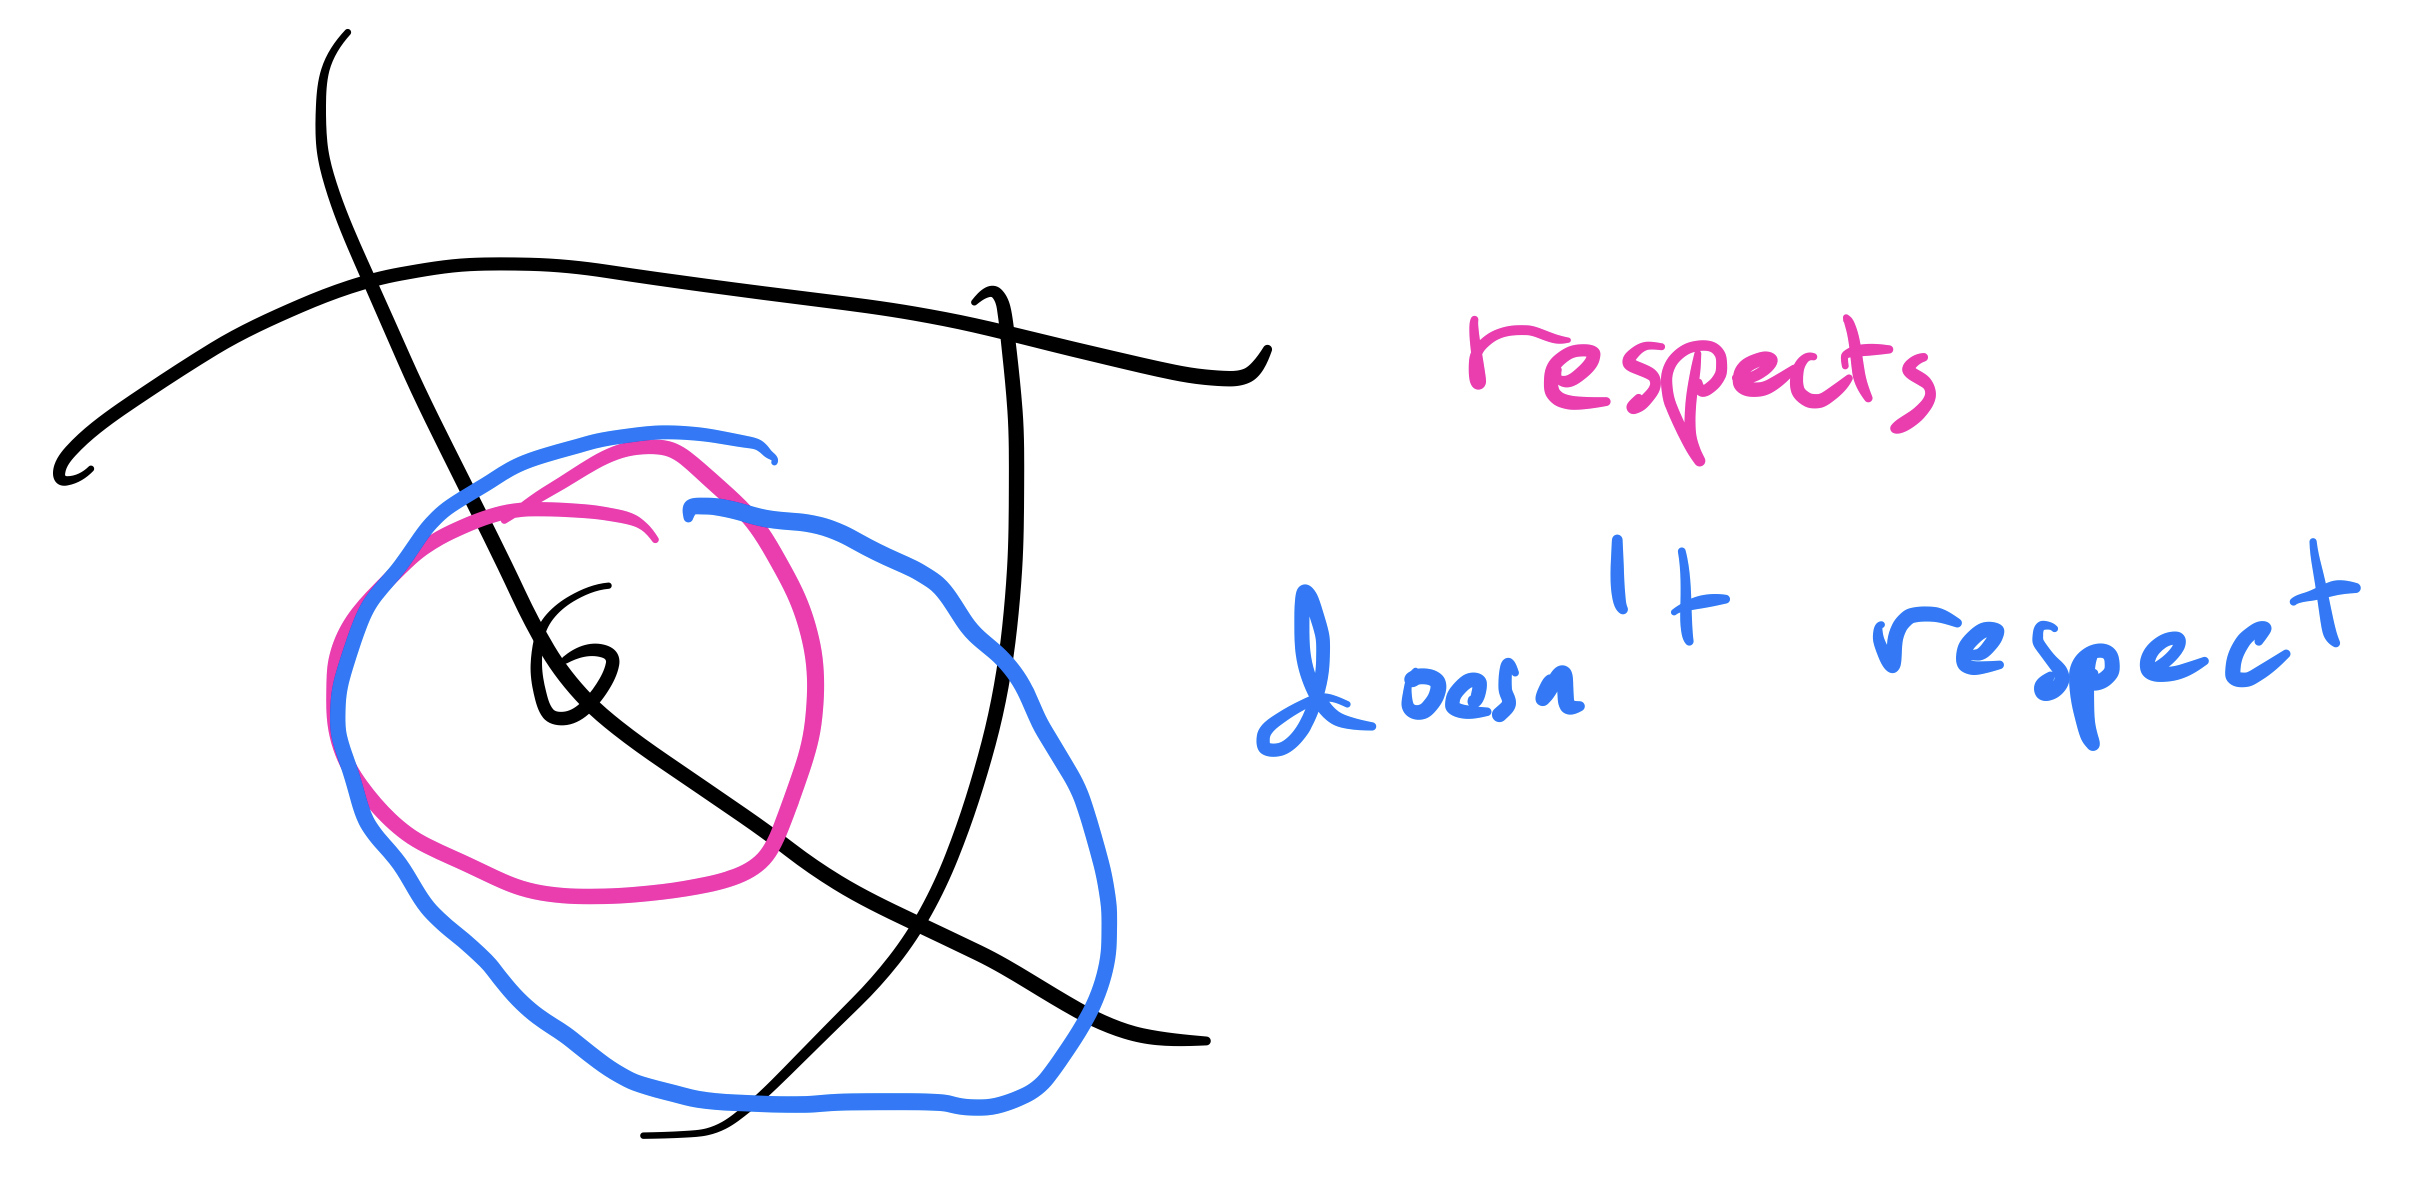
\includegraphics[width=0.5\textwidth]{images/figure-1.jpeg}

Every point has at least one such neighborhood (curves are compact). 
Let \(\mathcal{O}\) be the colection of all open neighborhoods of \(p\in C\) that respect 
the family \((C_i)_{i\in I}\). 

\(\mathcal{O}\) is an open cover of \(C\). \(\Rightarrow\) it contains a finite subcover 
\(\mathcal{O}'\) of \(C\). \(\Rightarrow\) each curve \(C_i\) is contained 
in a finite collection \(\mathcal{O}_i' \subseteq \mathcal{O}'\) of open sets
none of whom contain any points of curves \(C_j\) that \(C_i\) does not intersect. 

Replace \(C_i\) with a simple polygonal arc \(P_i\) in \(\mathcal{O}_i'\) 
while guaranteeing that \(P_i\) intersects \(P_j\) if \(C_i\) and \(C_j\) intersect.
(Possible since \(\exists O \in \mathcal{O}'\) which contains a common intersection point of \(C_i\) and \(C_j\)).
\end{proof}

\begin{lemma}
\begin{enumerate}
    \item \(c_w(m) \leq c_r(m)\)
    \item \( c_r(m) \leq 4 c_s(m^2 + 4m) \)
    \item \(c_s(m) \leq 4 c_w(2m) + 2m\)
\end{enumerate}
\end{lemma}

\begin{proof}
    TODO (page 4 of Decidability of string graphs paper)
\end{proof}

\begin{lemma}
    Every word of length \(\geq 2^n\) over an alphabet of size \(n\) contains a non-trivial subword in which every character occurs an even number of times.
\end{lemma}

\begin{proof}
TODO (Lemma 3.1 of Decidability of string graphs paper)
\end{proof}

\begin{theorem}
    Let \(G\) be a graph with \(m\) edges, \(R \subseteq \binom{E}{2}\) such that \((G, R)\) is weakly realizable, and let \(D\) 
    be a weak realization of \((G, R)\) with the minimal number of intersections. Then for any edge \(e \in G\) 
    there are less than \(2^m\) intersections on the curve realizing \(e\) in \(D\).
\end{theorem}

\begin{proof}
TODO (Theorem 3.2 of Decidability of string graphs paper)
\end{proof}

\begin{corollary}
    String graph recognition is in \textbf{NEXP}.
\end{corollary}

\begin{proof}
TODO (Corollary 3.3 of Decidability of string graphs paper)
\end{proof}

\end{document}
